\documentclass{beamer}

\usepackage[utf8]{inputenc}
\usepackage[T2A]{fontenc}
\usepackage[russian]{babel}
\usepackage{url}

\usepackage{amsmath}
\usepackage{tikz}
\usepackage{graphicx}
\usepackage{svg}

\usetheme{Madrid}

\defbeamertemplate*{title page}{customized}[1][]
{
    \begin{center}
        \usebeamerfont{title}
        \inserttitle
        \par
    \end{center}
    \bigskip
    \hfill
    \hbox{
        \usebeamerfont{author}
        \begin{tabular}{ll}
            Студент: & Суркис Антон Игоревич \\
            Научный руководитель: & Попов Иван Александрович \\
        \end{tabular}
    }
    \par
    \begin{center}
        \usebeamerfont{date}
        \insertdate
        \par
    \end{center}
}

\title{Исследование границ применимости процедурного кластерного видозависимого лоддирования в современных компьютерных играх}
\author{Антон Суркис}

\begin{document}
    \maketitle

    \begin{frame}{Введение}
        \begin{itemize}
            \item
            В современных компьютерных играх для реалистичной графики
            используют высокодетализированные модели объектов;

            \item
            Отрисовывать такие высокодетализированные модели для
            всех объектов на экране очень долго,
            а компьютерная игра должна реагировать на ввод
            в реальном времени;

            \item
            Стандартное решение --- рисовать объекты
            далеко от камеры в заранее заготовленной
            менее детализированной версии;

            \item
            Такие менее детализированные версии
            сложно и дорого создавать и применять;

            \item
            Выбор уровня детализации для объекта целиком
            плохо работает для больших объектов,
            например, статуй и зданий,
            у которых одна часть может оказаться близко
            к камере, а другая --- далеко.
        \end{itemize}
    \end{frame}

    \begin{frame}{Введение}
        \begin{itemize}
            \item Было много попыток создать альтернативу
            статическим уровням детализации, например,
            Sparse Voxel Octrees и мегатекстуры
            от~id~Software;

            \item В 2020 году компания Epic Games представила
            существенно другой подход к оптимизации
            отрисовки высокодетализированных объектов
            --- технологию Nanite в движке Unreal Engine 5.
            Nanite:
            \begin{itemize}
                \item Генерирует все уровни детализации автоматически,
                без ручной обработки;
                \item Отображает части объекта с разной детализацией;
                \item Делает швы между разными уровнями детализации незаметными;
                \item Отображает максимальную детализацию,
                для которой хватает разрешения экрана.
            \end{itemize}
        \end{itemize}
    \end{frame}

    \begin{frame}{Проблема}
        \begin{itemize}
            \item Несмотря на все эти преимущества и то,
            что Nanite представили ещё в 2020,
            а описание его работы открыто,
            далеко не все движки внедрили подобные технологии.
            За 4 года в свои движки технологию НЕ внедрили:
            \begin{itemize}
                \item Unity
                \item Activision
                \item Ubisoft
                \item Crytek
                \item CD Projekt Red
                \item и т.д.
            \end{itemize}

            \item Следовательно, у технологии есть
            какие-то значительные недостатки,
            сравнимые с преимуществами.
        \end{itemize}
    \end{frame}

    \begin{frame}{Цели и задачи}
        \textbf{Цель работы:}
        исследовать ограничения динамической кластерной детализации,
        существенные для компании-разработчика игр.

        \bigskip

        \textbf{Задачи:}
        \begin{itemize}
            \item Изучить механизм работы Nanite;
            \item Реализовать упрощённую систему
            динамической кластерной детализации;
            \begin{itemize}
                \item Одна из гипотез --- Nanite
                очень сложен в реализации,
                для её проверки предлагается реализовать
                упрощённую версию;
            \end{itemize}
            \item Определить проблемы, возникающие при реализации;
            \item Определить принципиальные ограничения технологии;
            \item Сравнить с ,,монолитной`` детализацией.
        \end{itemize}
    \end{frame}

    \begin{frame}{Nanite}
        Общий механизм работы
        Nanite\footnote{
            \url{https://advances.realtimerendering.com/s2021/Karis_Nanite_SIGGRAPH_Advances_2021_final.pdf}
        } состоит из двух этапов:
        \begin{itemize}
            \item Предподсчёт --- преобразование модели;
            \item Непосредственно отрисовка.
        \end{itemize}
    \end{frame}

    \begin{frame}{Nanite: предподсчёт}
        \begin{itemize}
            \item Один объект разбивается на
            стыкующиеся между собой маленькие объекты
            --- ,,мешлеты`` (meshlet);
            \item Из исходных мешлетов создаются
            мешлеты с меньшей детализацией;
            \item Все мешлеты вместе образуют ациклический
            направленный граф;
            \item \textbf{При спуске по графу
            оценка искажения от исходной модели уменьшается;}
            \item Стоки этого графа --- исходные мешлеты,
            полученные при разбиении,
            их оценка ошибки строго нулевая.
        \end{itemize}
    \end{frame}

    \begin{frame}{Nanite: пример предподсчёта, шаг 1}
        \centering
        \includesvg{metis-0.svg}
    \end{frame}

    \begin{frame}{Nanite: пример предподсчёта, шаг 2}
        \centering
        \includesvg{metis-1.svg}
    \end{frame}

    \begin{frame}{Nanite: пример предподсчёта, шаг 3}
        \centering
        \includesvg{metis-2.svg}
    \end{frame}

    \begin{frame}{Nanite: пример предподсчёта, шаг 4}
        \centering
        \includesvg{metis-3.svg}
    \end{frame}

    \begin{frame}{Nanite: отрисовка}
        \begin{itemize}
            \item \textbf{Решение рисовать мешлет или нет
            принимается независимо от остальных мешлетов;}
            \item Это позволяет добиться массового параллелизма
            на видеокарте;
            \item Новые видеокарты аппаратно поддерживают отрисовку
            массивов мешлетов наравне с массивами треугольников;
            \item Для видеокарт, не поддерживающих мешлеты аппаратно,
            можно их реализовать программно;
            \item Маленькие треугольники (размером 1 пиксель)
            рисуются с помощью вычислительного шейдера:
            \begin{itemize}
                \item Таких треугольников большинство
                при высокой детализации исходной модели,
                поэтому их надо учитывать;
                \item Пиксельные шейдеры в видеокартах
                на такое не рассчитаны --- они всегда
                обрабатывают минимум квадрат 2 на 2 пикселя.
            \end{itemize}
        \end{itemize}
    \end{frame}

    \begin{frame}{Реализация}
        Для реализации использовал DirectX 12:
        \begin{itemize}
            \item DirectX 12 поддерживает технологию Mesh Shader,
            т.е. отрисовку массивов мешлетов;
            \item Также можно было бы использовать Vulkan
            с расширением \texttt{VK\_EXT\_mesh\_shader},
            но проект DirectX 12 оказался проще в настройке;
            \item Средство отладки PIX поддерживает отладку
            таких шейдеров, в отличие от RenderDoc;
            \item DirectX 11 не поддерживает Mesh Shader;
            \item По OpenGL 4 не удалось найти информации
            об официальных расширениях,
            только о расширении NVidia
            \texttt{GL\_NV\_mesh\_shader};
            \item Поддержка Mesh Shader в API не необходима
            для реализации, но значительно её упрощает.
        \end{itemize}
    \end{frame}

    \begin{frame}{Проблемы при реализации}
        Значительные проблемы возникли при кластеризации:
        \begin{itemize}
            \item Nanite использует библиотеку METIS
            для кластеризации треугольников;
            \item Алгоритм в этой библиотеке --- стохастический;
            \item У технологии Mesh Shader есть жёсткое ограничение
            на размер мешлета;
            \item METIS такое ограничение задать не позволяет;
            \item Решение, которое используют в Nanite
            --- задать целевой размер мешлета меньше
            жёсткого ограничения и надеяться,
            что METIS не выдаст слишком неравномерную кластеризацию;
            \item Иногда эти надежды не оправдываются.
        \end{itemize}
    \end{frame}

    \begin{frame}{Проблемы при реализации: кластеризация}
        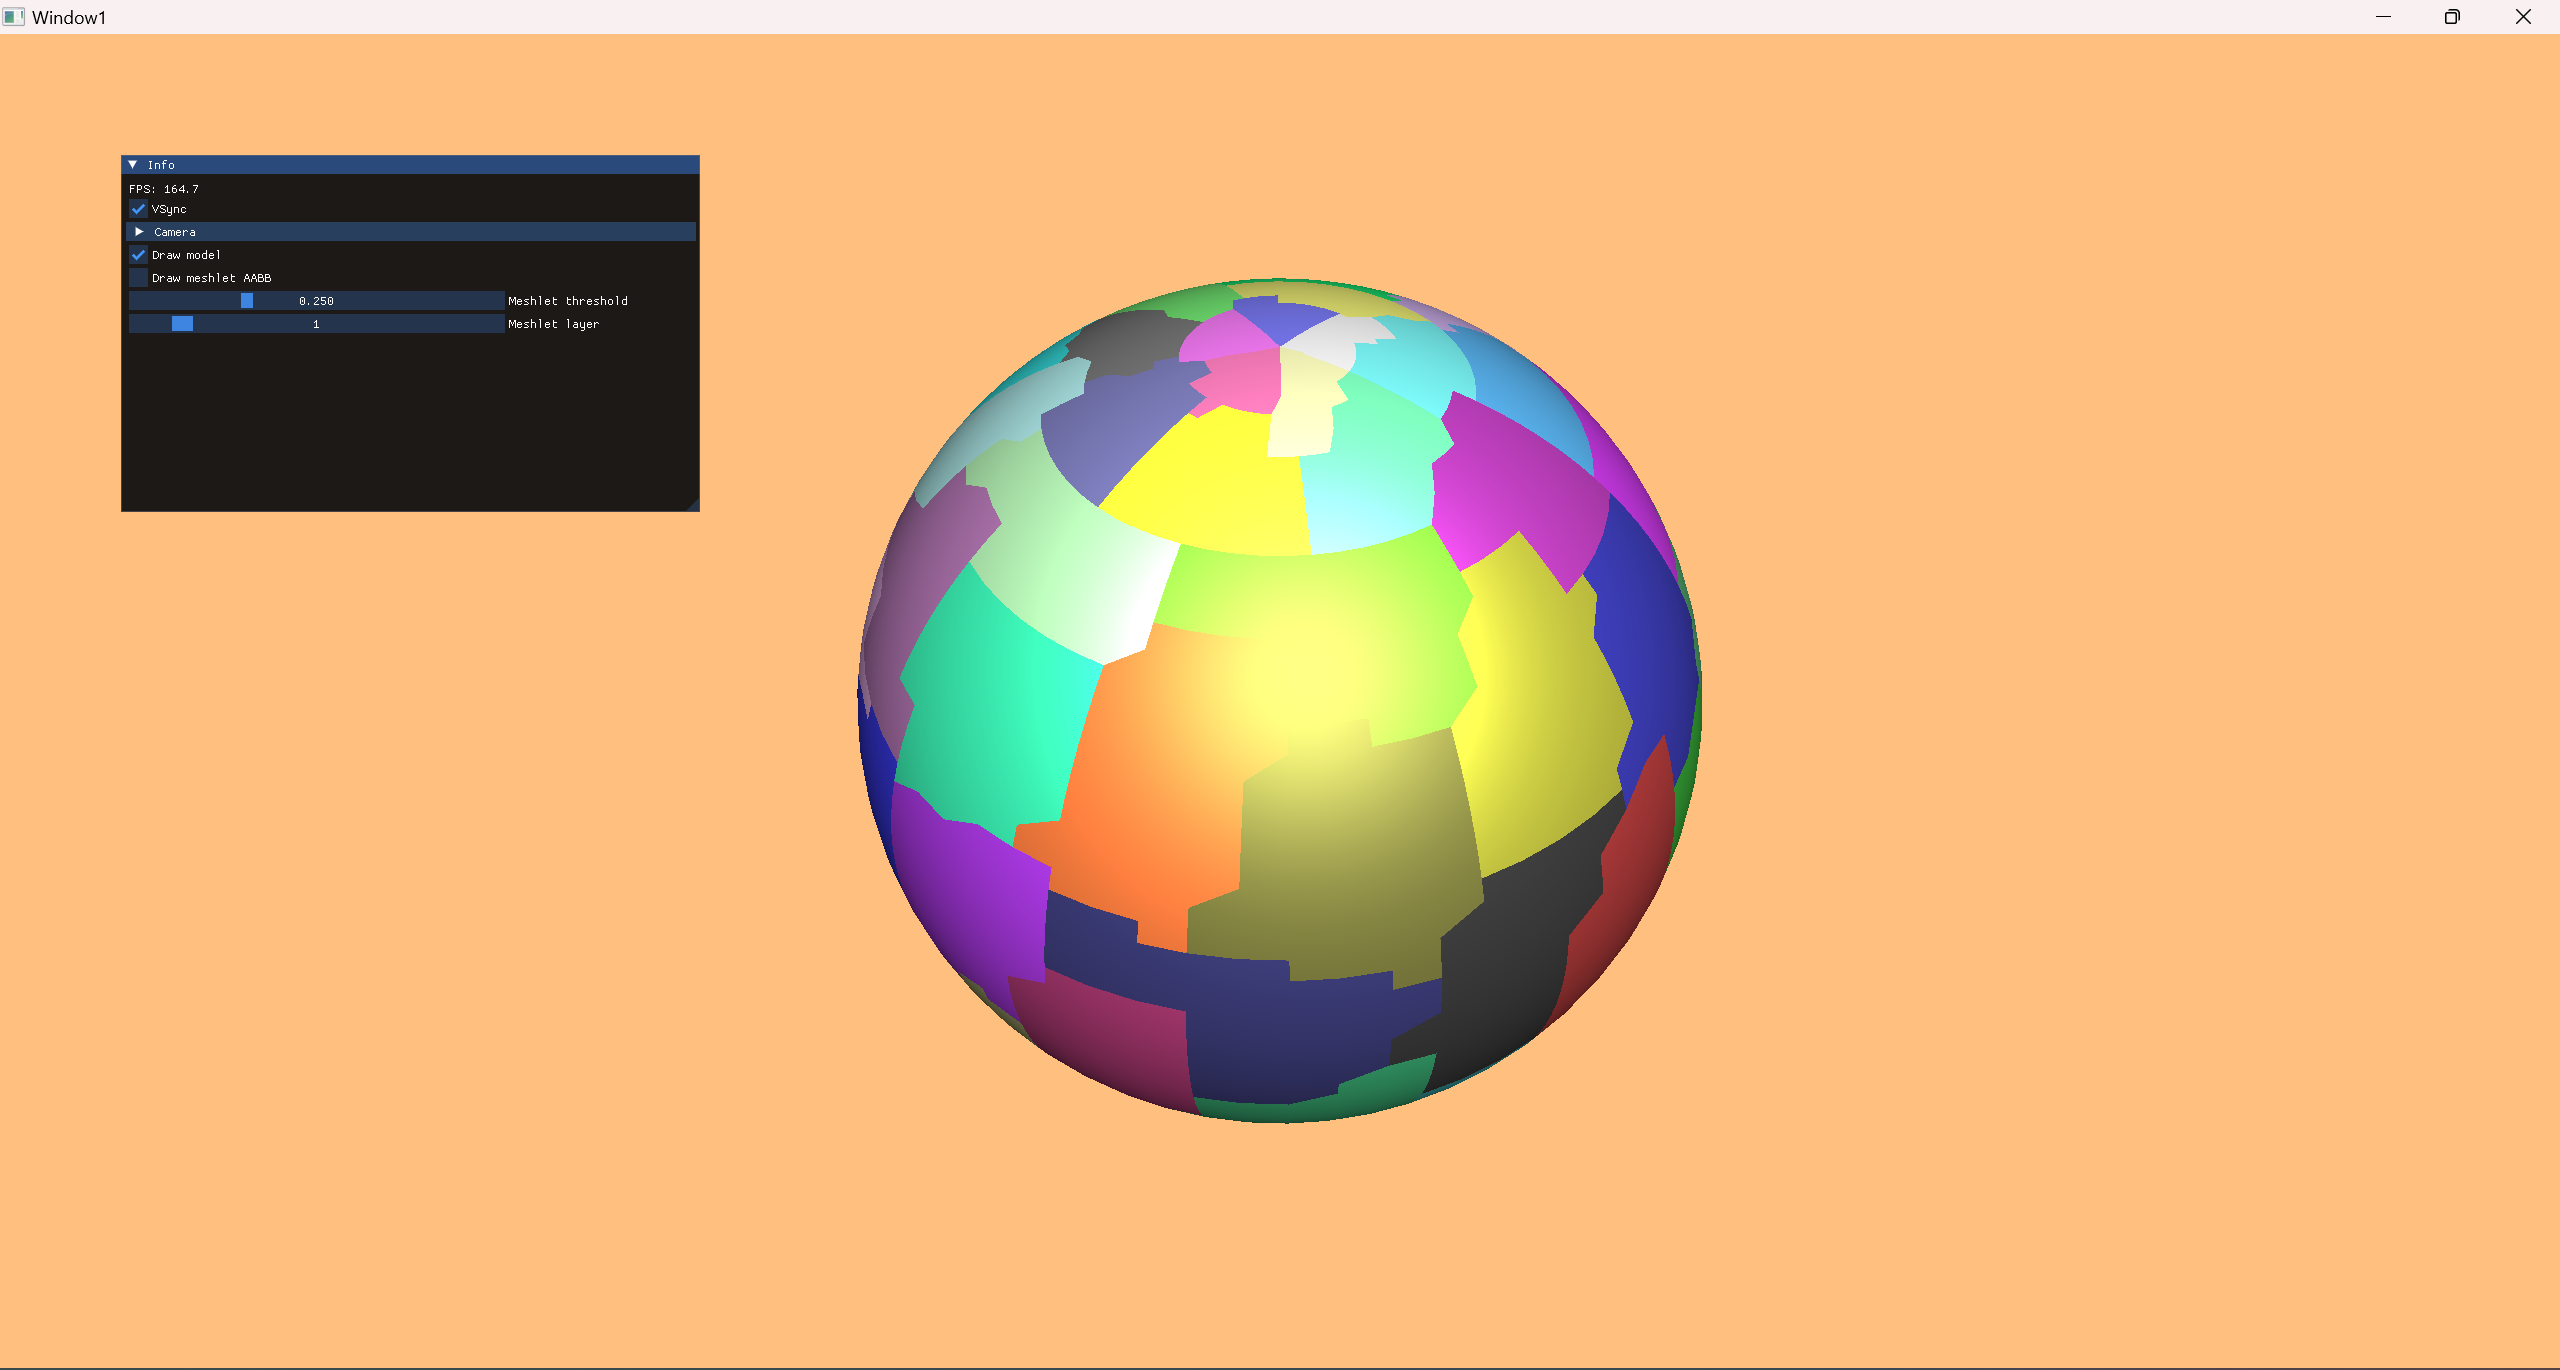
\includegraphics[width=\textwidth]{sphere0.png}
    \end{frame}

    \begin{frame}{Проблемы при реализации: последствия}
        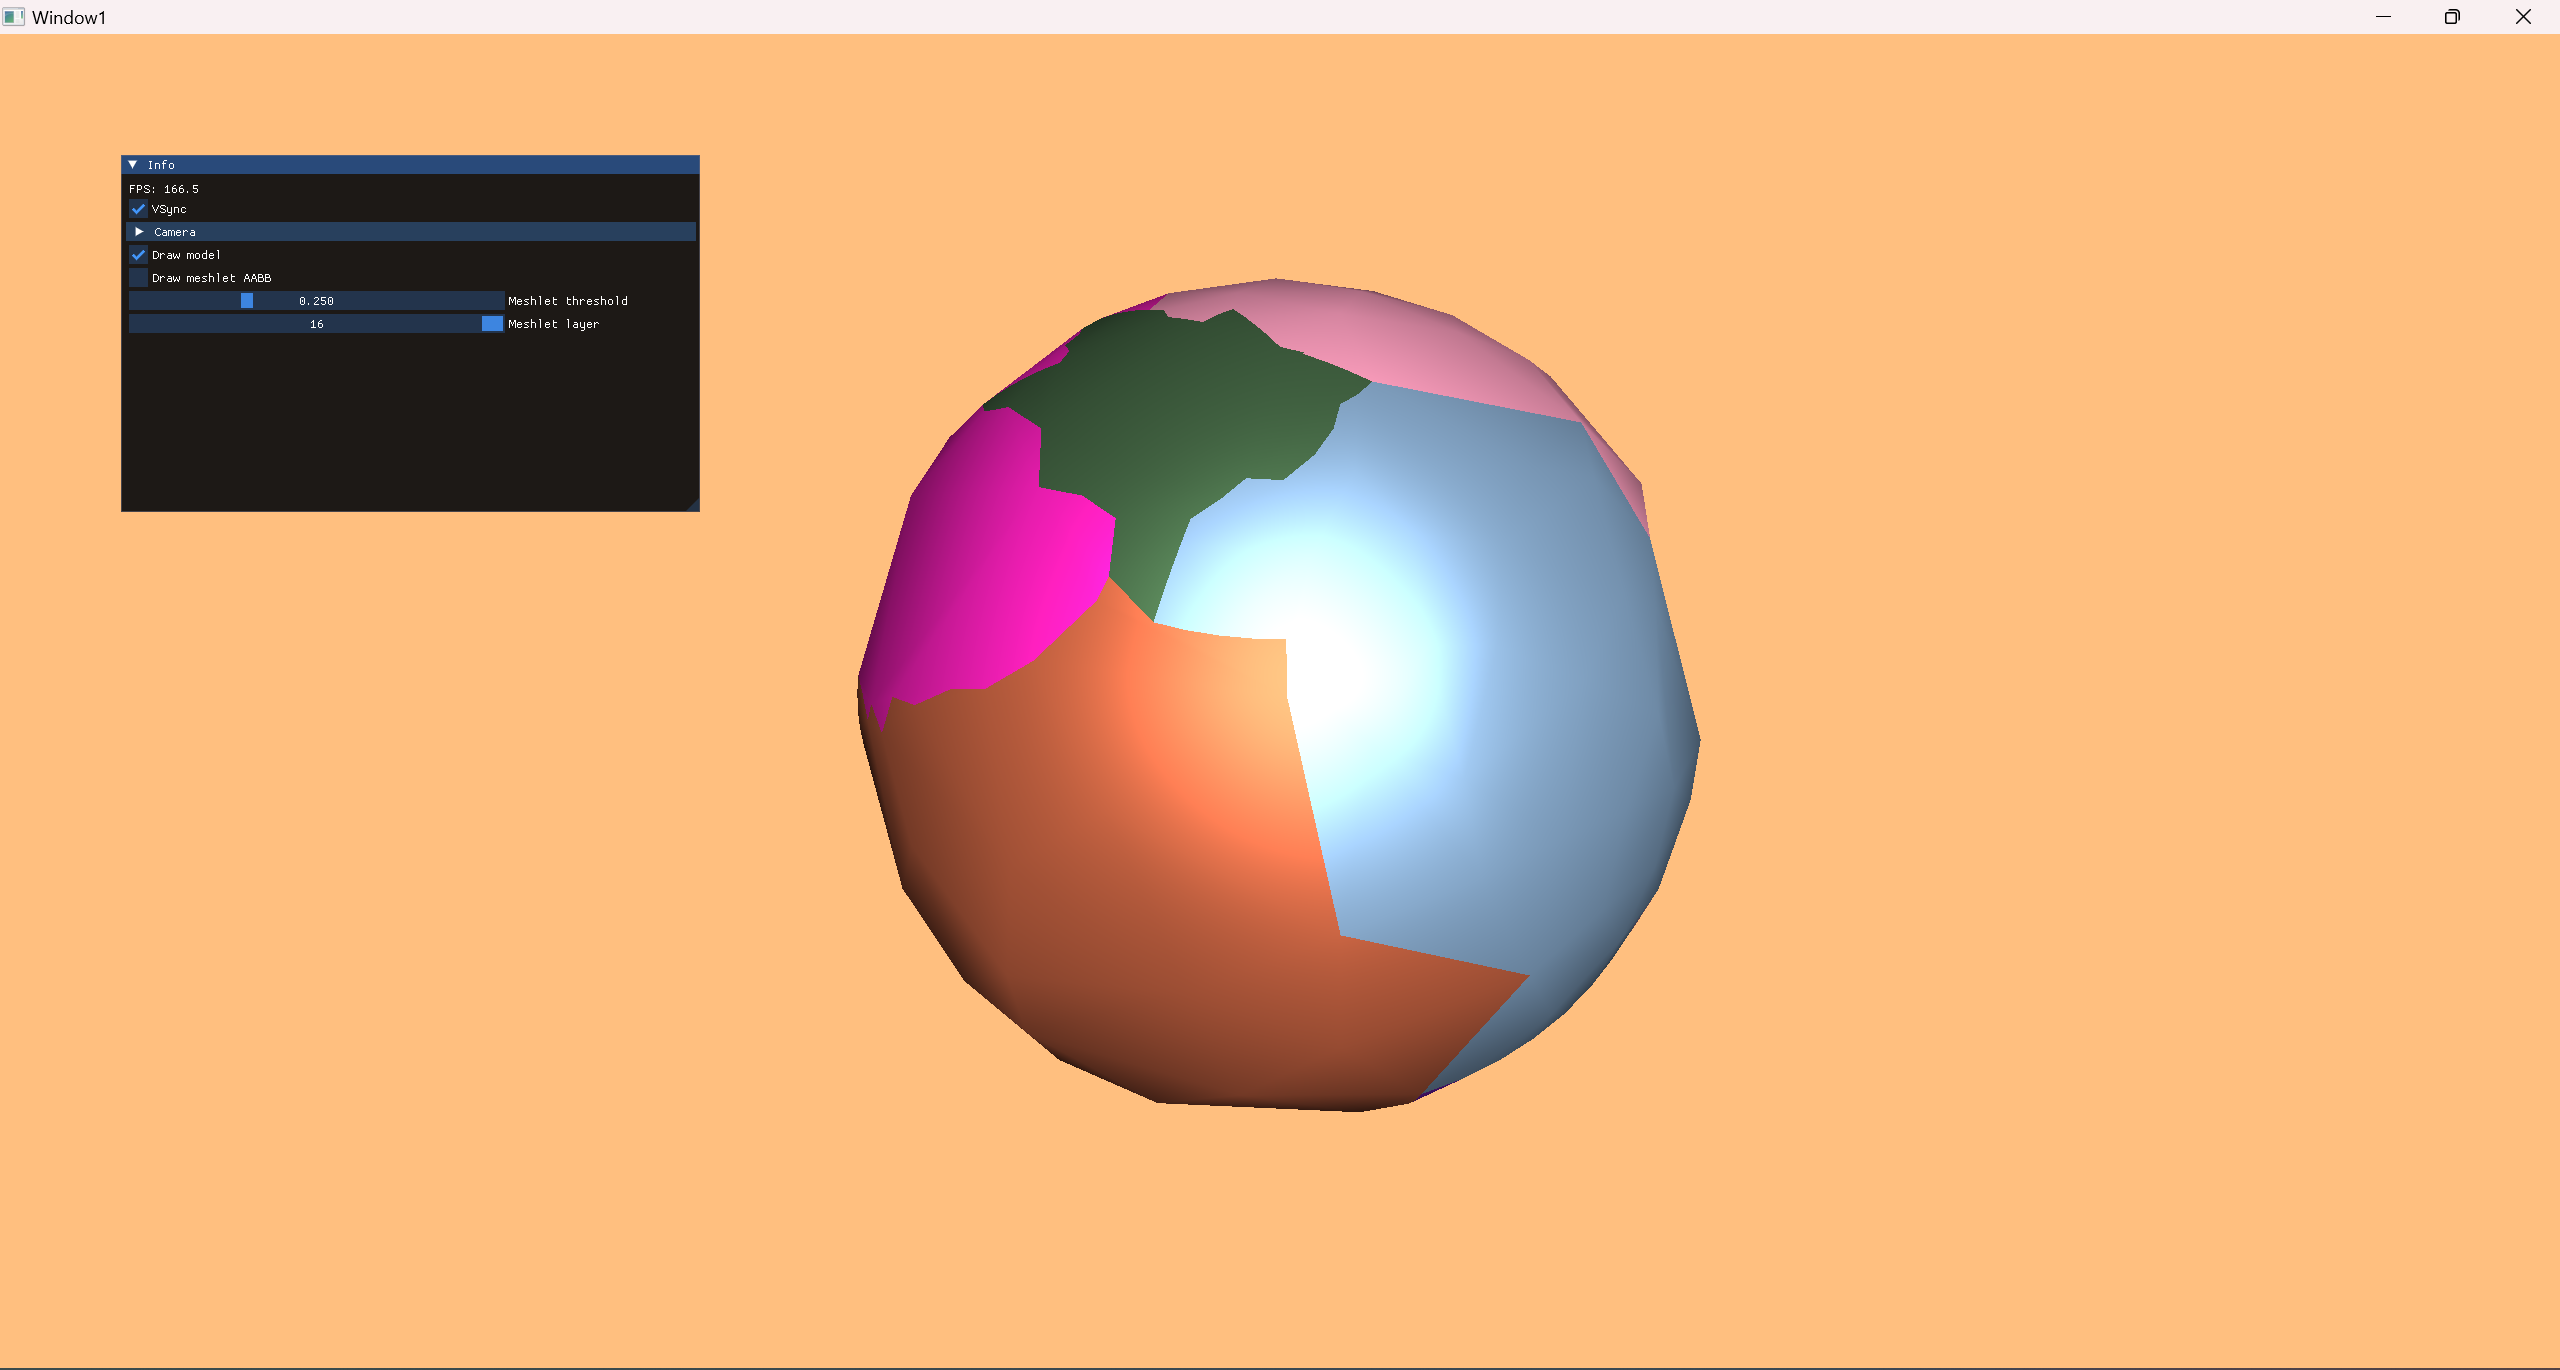
\includegraphics[width=\textwidth]{sphere1.png}
    \end{frame}

    \begin{frame}{Принципиальные ограничения}
        \begin{itemize}
            \item
            В оценке искажения учитывается расстояние
            от мешлета до камеры,
            но невозможно учесть направление взгляда.
            Из-за этого часто Nanite приходится
            рисовать избыточную детализацию.

            \item
            При любом движении вершин исходной модели
            друг относительно друга оценки искажения
            станут некорректными, из-за этого
            может сломаться переключение детализации.
            Поэтому технология применима только
            к статичной геометрии;

            \item
            Кластеризация треугольников и последующее уменьшение
            детализации сильно завязаны на то,
            что исходная модель --- поверхность замкнутого объёма.
            Основная часть крупных объектов в компьютерных играх
            попадают под такое определение.
        \end{itemize}
    \end{frame}

    % \begin{frame}{Принципиальное ограничение: поддержка}
    %     Mesh Shader появились сравнительно недавно,
    %     например, видеокарты NVidia поддерживают
    %     их только начиная с 20xx серии.
    %     Согласно статистике Steam на март 2024,
    %     32\% используемых игроками видеокарт NVidia
    %     --- более ранних серий,
    %     это 23\% от всех устройств.

    %     Как уже было упомянуто ранее,
    %     можно использовать мешлеты без Mesh Shader,
    %     но для этого придётся поддерживать две версии
    %     движка --- для старых и для новых видеокарт.

    %     \bigskip

    %     Однако стоит разделять
    %     23\% от тех компьютеров,
    %     с которых была собрана статистика,
    %     и 23\% всех игроков ---
    %     часть игроков имеет несколько компьютеров,
    %     часть отказывается от сбора статистики,
    %     а для части игроков основная платформа
    %     --- игровая консоль, а не персональный компьютер.
    % \end{frame}

    \begin{frame}{Принципиальное ограничение: объём}
        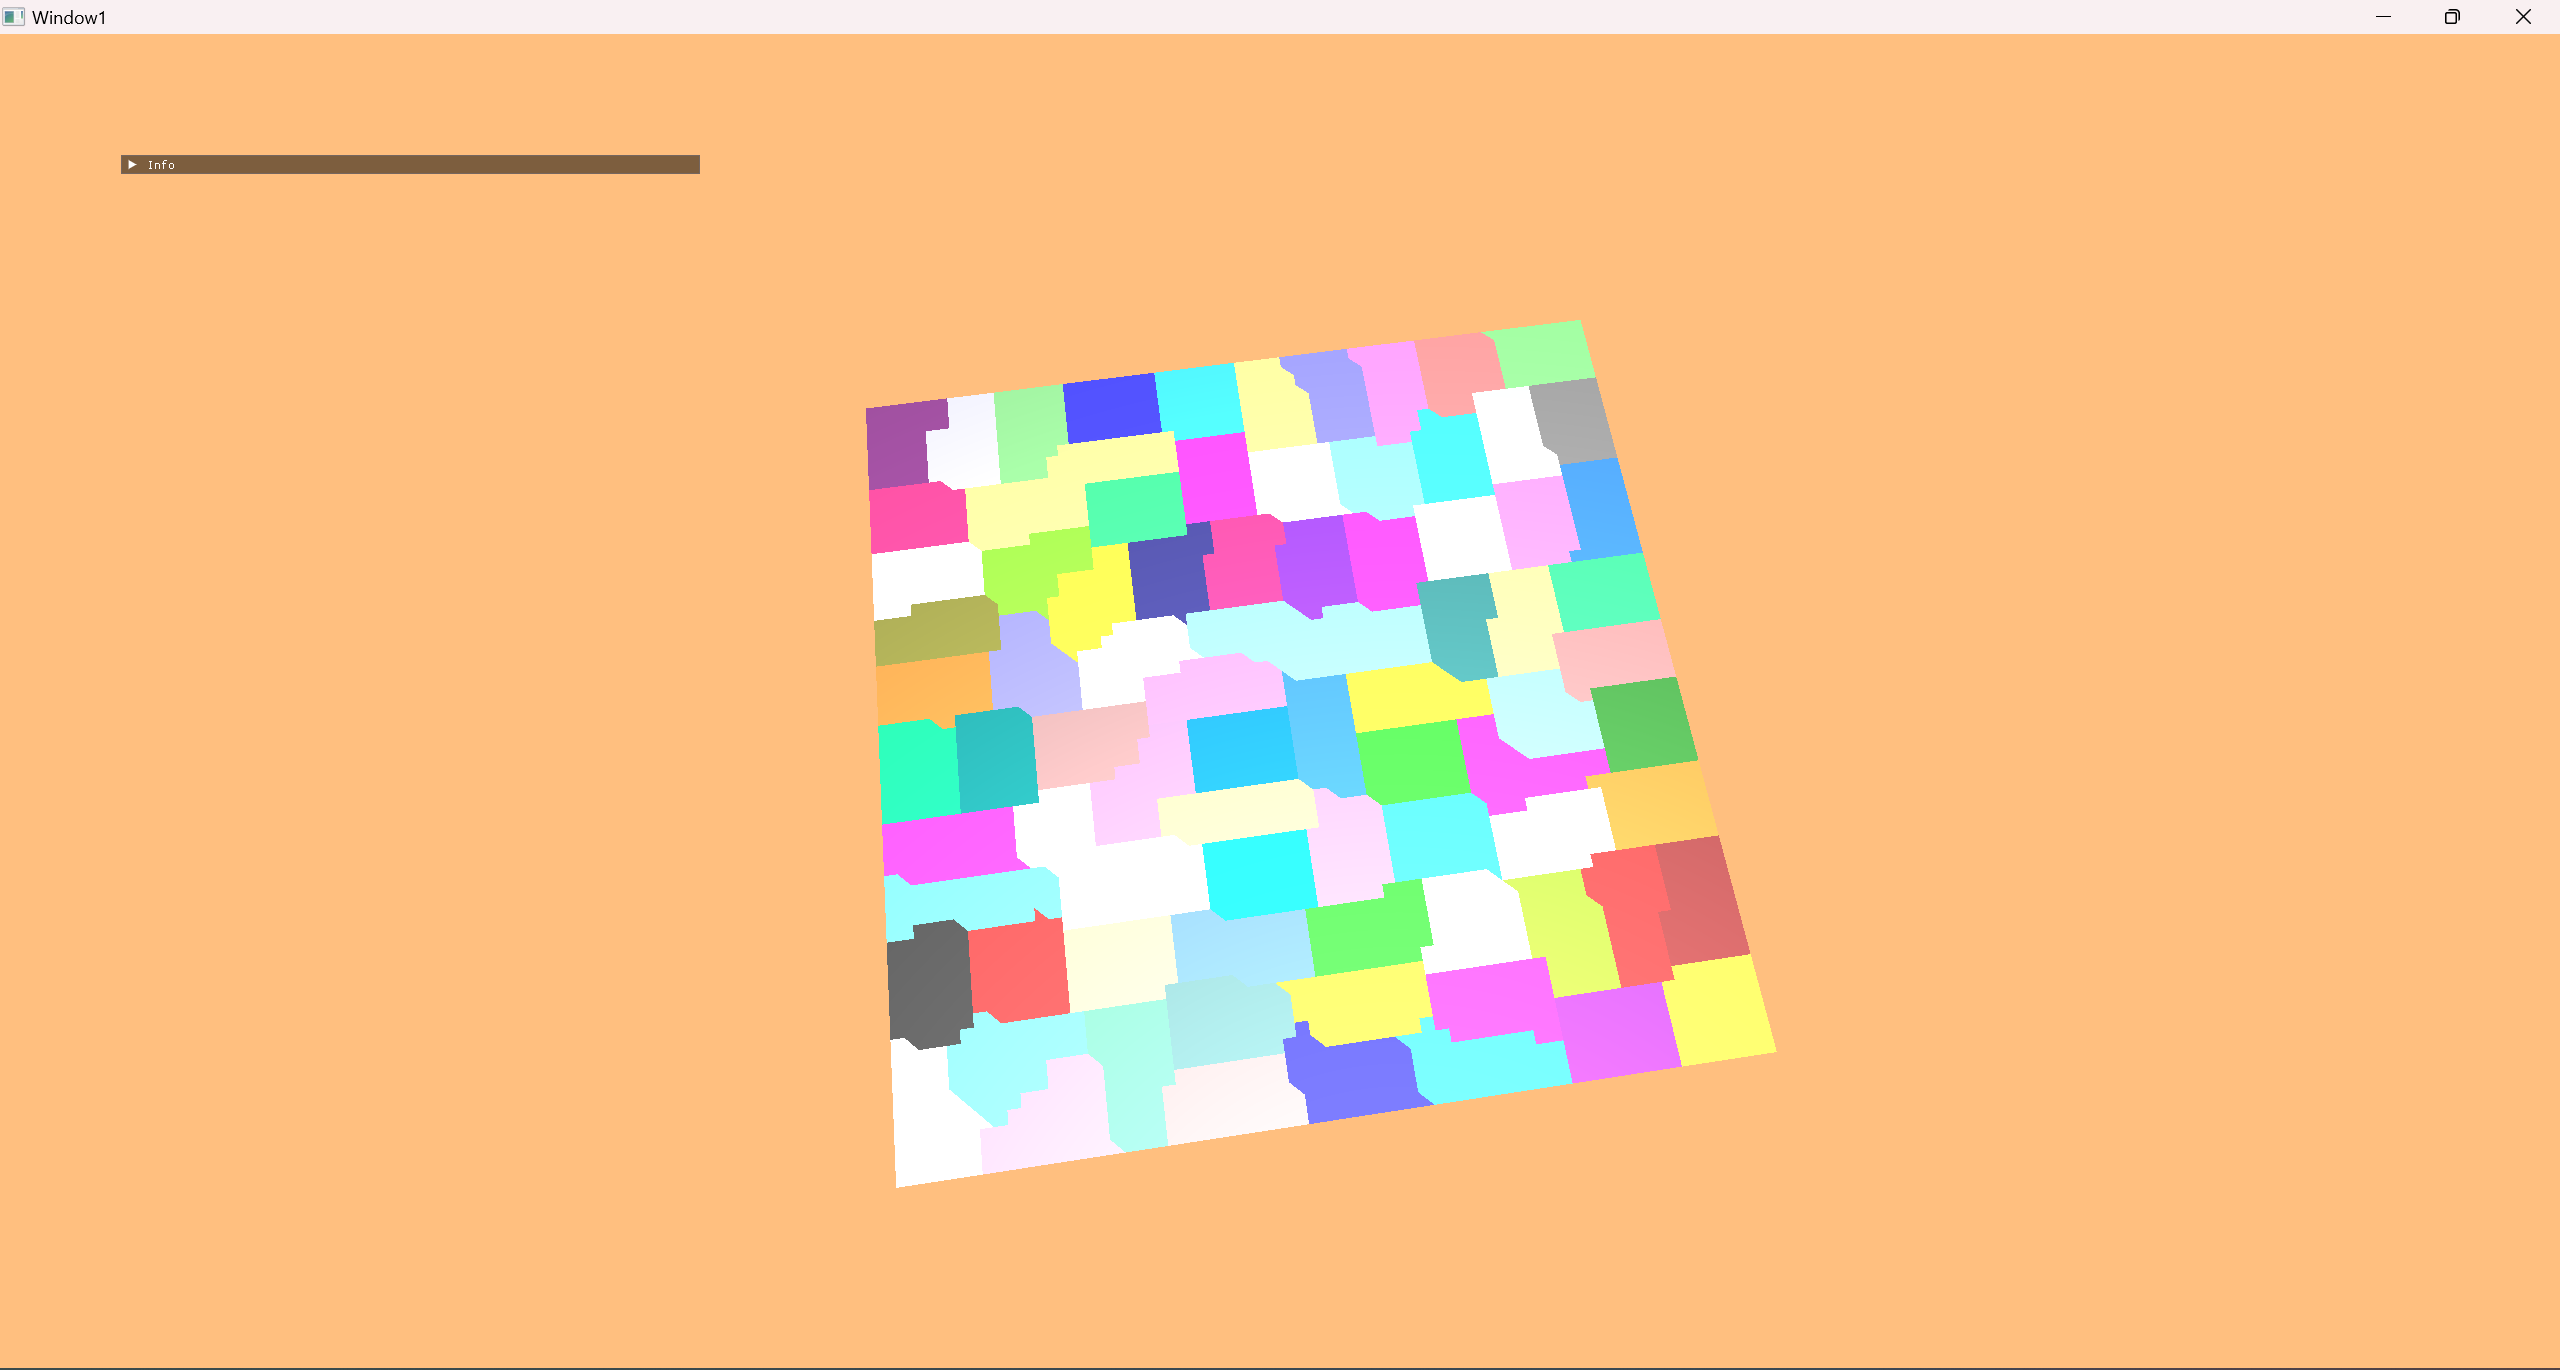
\includegraphics[width=\textwidth]{plane0.png}
    \end{frame}

    \begin{frame}{Принципиальное ограничение: объём}
        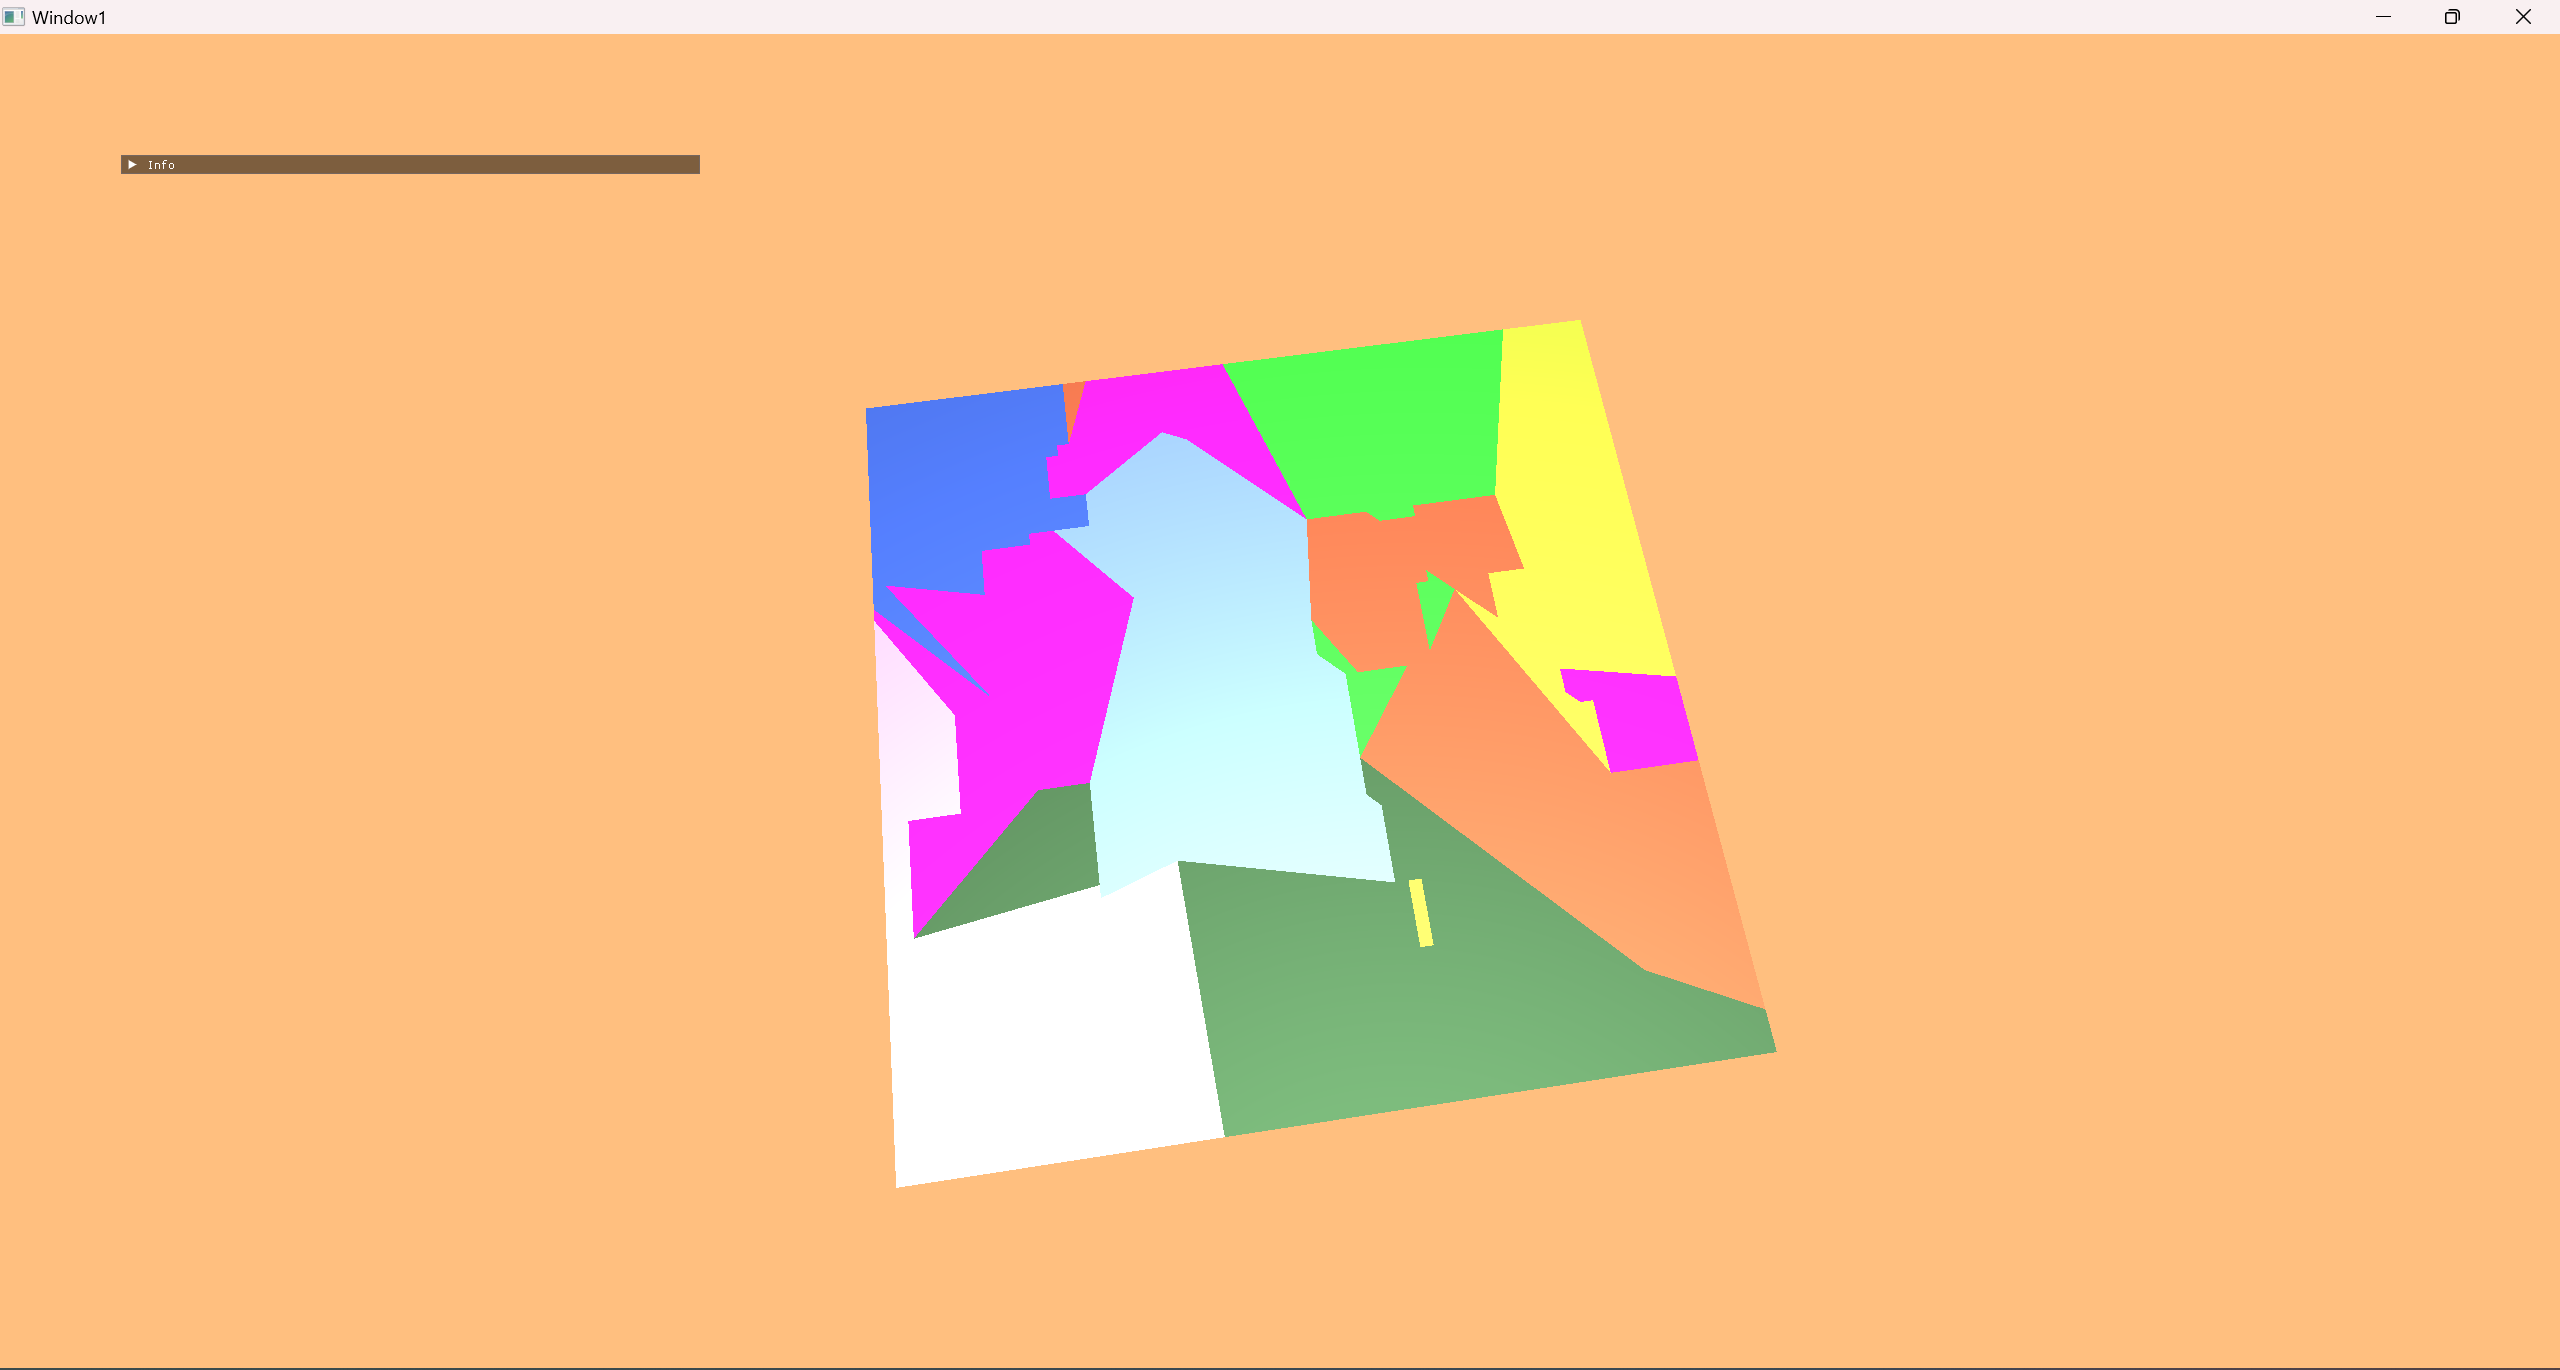
\includegraphics[width=\textwidth]{plane1.png}
    \end{frame}

    \begin{frame}{Сравнение с некластерной детализацией}
        Пока не проводилось
    \end{frame}

    \begin{frame}{Результаты}
        \begin{itemize}
            \item Выявлены существтенные проблемы,
            возникающие при реализации
            динамической кластерной детализации;

            \item Выявлены принципиальные
            ограничения технологии,
            которые существенны при принятии решения
            о реализации полной, а не упрощённой,
            версии и интеграции в существующий движок.
        \end{itemize}
    \end{frame}
\end{document}
